\chapter*{Appendix}

\section{Geometric approach to multi parametric programming}\label{BASICCSR:sec:MPP}
    % Section's main text due to more comprehensible source

    In this section the goal is to explain how to solve multi-parametric optimization problems (mp-OP). By start lets consider the following linear multip-parametric problem:

        \begin{equation}
    \begin{array}{rcl}
            J^*(\textbf{x})&=&\min_{\textbf{z}}J(\textbf{x},\textbf{z})=\textbf{c}'\textbf{z}\\
            %&=&\frac{1}{2}\textbf{z}'\textbf{H}\textbf{z}\\
            &\textnormal{subj. to}&\textbf{Gz}\leq\textbf{w}+\textbf{Sx},
        \end{array}
        \label{BASICMPC:equ:MPP_program}
    \end{equation}

    where $\textbf{z}\in\mathbb{R}^s$ is the vector of the optimization variables,  $\textbf{x}\in\mathbb{R}^n$ is the vector of parameters, and of course $J(\textbf{x},\textbf{z}):\mathbb{R}^{s+n}\rightarrow\mathbb{R}$ is the objective or cost function. Additionally $\textbf{G}\in\mathbb{R}^{m\cdot s}$, $\textbf{w}\in\mathbb{R}^m$, $\textbf{c}\in\mathbb{R}^s$ and $\textbf{S}\in\mathbb{R}^{m\cdot n}$ as described in section \ref{BASICCSR:sec:OptimalControl}. Next we define a closed convex parameter set $\textbf{K}\subset\mathbb{R}^n$ such as:

    \begin{equation}
    \begin{array}{rcl}
            \textbf{K}&=&\left\{ \textbf{x}\in\mathbb{R}^n:\textbf{Tx}\leq\textbf{Z}\right\},
        \end{array}
        \label{BASICMPC:equ:MPP_parameterset}
    \end{equation}

    where $\textbf{K}^*\subseteq\textbf{K}$ is the set where \ref{BASICMPC:equ:MPP_program} is feasible, and $\textbf{x}^*\in\textbf{K}^*$ where $\textbf{x}^*$ is the optimum. It is further assumed that:

    \begin{enumerate}
    \item the constraint $\textbf{x}\in\textbf{K}$ is included in the constraints of $\textbf{Gz}\leq\textbf{w}+\textbf{Sx}$.
    \item $\textbf{K}$ is a full dimensional polytope, or the problem can be reformulated to $\textbf{K}$ to be full dimensional with a smaller set of parameters.
    \item $\textbf{S}$ is on full rank, or the problem can be reformulated to $\textbf{S}$ to be full rank with a smaller set of parameters.
    \end{enumerate}

    As such $\textbf{J}^*:\textbf{K}^*\rightarrow\mathbb{R}$ is a function which gives the optimum by $\textbf{x}$. That said let $\textbf{Z}^*:\textbf{K}^*\rightarrow\mathbb{R}^s$ the function which gives the set of optimizers namely $\textbf{z}^*\in\textbf{Z}^*$. The task is to find a $\textbf{K}^*\subseteq\textbf{K}$ set and a $\textbf{z}^*\in\textbf{Z}^*$ optimizer and the value of the optimum.\\
    Beside of the systematic linear and quadratic program solutions \cite{borrelli2017predictive} there is a direct geometrical solution for the problem which uses critical regions for describing the parameter space. The critical regions are convex subsets of the parameter space where the optimum is constant based on the function of the parameters.
    Consider the multi parametric program \ref{BASICMPC:equ:MPP_program}, and let $\mathcal{I}_c=\{1,\dots,m\}$ be the set of constraint indices. For any $\mathcal{A}\subseteq\mathcal{I}_c$, let $\textbf{G}_{\mathcal{A}}$, and $\textbf{S}_{\mathcal{A}}$ be the subsets of $\textbf{G}$, and $\textbf{S}$, respectively, compromising the rows indexed by $\mathcal{A}$, and denote with $\textbf{G}_j$, $\textbf{S}_j$ and $\textbf{w}_j$, the $j^{th}$ row of $\textbf{G}$, $\textbf{S}$ and $\textbf{w}$. We define $\mathcal{C}_{\mathcal{A}}$ as the set of states $\textbf{x}$ for which the same set $\mathcal{A}$ of constraints is active at the optimum. Formally, the \emph{optimal partition} of $\mathcal{I}_c$ at $\textbf{x}$ is the optimal partition of $(\mathcal{A}(x),\mathcal{A}^N(x))$, where:

    \begin{equation}
    \begin{array}{rcl}
            \mathcal{A}&=&\{j\in\mathcal{I}_c:\textbf{G}_j\textbf{z}^*(x)-\textbf{S}_j\textbf{x}=\textbf{w}_j\forall\textbf{z}^*\in\textbf{Z}^*(x)\}\\
            \mathcal{A}^N&=&\{j\in\mathcal{I}_c:\exists\textbf{z}^*\in\textbf{Z}^*(x)\textnormal{ s.t.: }\textbf{G}_j\textbf{z}^*(x)-\textbf{S}_j\textbf{x}<\textbf{w}_j\}.
        \end{array}
        \label{BASICMPC:equ:MPP_stateset_optimal partition}
    \end{equation}

    It can be noticed, that $\mathcal{A}$ and $\mathcal{A}^N$ are disjoint (the intersection of $\mathcal{A}$ and $\mathcal{A}^N$ is an empty set) and they union is $\mathcal{I}_c$. As such consider a set $\mathcal{A}\subseteq\mathcal{I}_c$, then the \emph{critical region} associated with the set of active constraints $\mathcal{A}$ is defined as:

    \begin{equation}
    \begin{array}{rcl}
            \mathcal{C}_{\mathcal{A}}&=&\{\textbf{x}\in\textbf{K}^*:\mathcal{A}(x)=\mathcal{A}\}.
        \end{array}
        \label{BASICMPC:equ:MPP_stateset_optimal critical}
    \end{equation}

    With the above the critical region $\mathcal{C}_{\mathcal{A}}$ is the set of all $\textbf{x}$ states such that constraints indexed by $\mathcal{A}$ are active at the optimum of problem \ref{BASICMPC:equ:MPP_program}. Furthermore it can be proven, that the optimum is an affine function in the domain of $\textbf{K}$ adn unique for every critical region. As such the problem can be separated into two parts:

    \begin{enumerate}
    \item Find the least dimension subset of $\textbf{K}$ which contains $\textbf{K}^*$.
    \item Partition $\textbf{K}^*$ into critical regions and find the optimum for every critical region.
    \end{enumerate}

    The graphical representation of critical regions can be observed at Fig.\ref{BASICCSR:fig:Crit}. The algorithm starts from a starting point $\textbf{x}_0$ and solves the linear programming problem and find $\textbf{z}^*(\textbf{x}_0)$. After this find the active constrains and define the corresponding critical region $\mathcal{C}_{\mathcal{A}}(\textbf{x}_0)$. Its clear from the definition of one critical region that $J^*$ is constant for any $\textbf{x}\in\mathcal{C}_{\mathcal{A}}(\textbf{x}_0)$. Next  we find the optimum and the optimizer's value for $\textbf{x}\in\mathcal{C}_{\mathcal{A}}(\textbf{x}_0)$. and move on to the next critical region. If the optimum problem is not degenerate then finding the critical regions is straightforward, but in the contrary the outcome is defined by the algorithm's starting direction.

    \begin{figure}[!ht]
        \centering
        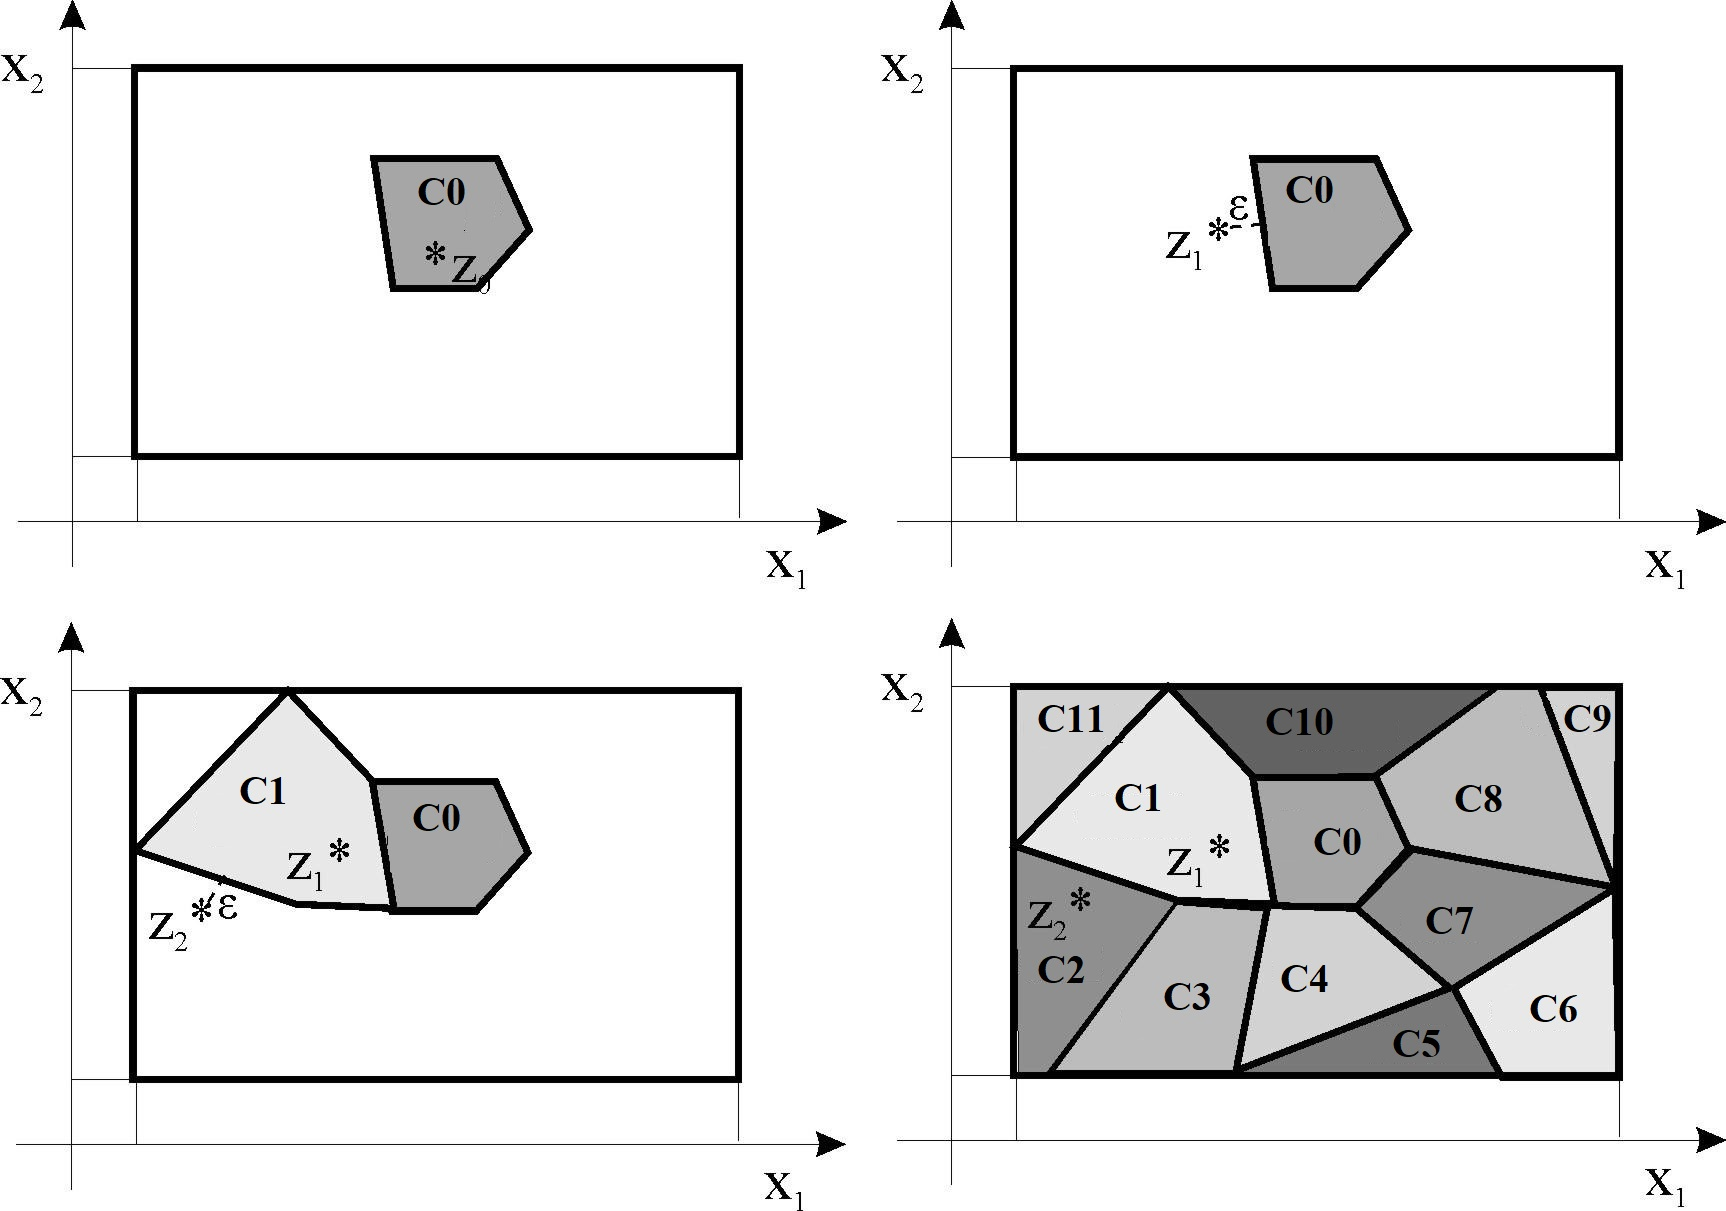
\includegraphics[width=.9\textwidth]{EMPC_PNG_Pics/criticalregions.jpg}
        \caption{Partitioning incrementally the two dimensional parameter space to critical regions from $C0$ to $C11$.}
        \label{BASICCSR:fig:Crit}
    \end{figure}

    As it shall be described in section \oldref{EMPC:sec:main}, the if the linear optimization could be described with quadratic programming the process yield more computational cost efficient results in a lot of cases. As such it is advised to apply above geometrical approach in a multi-parametric quadratic programming (mp-QP) environment, as it would be used in the explicit MPC. Consider a multi parametric quadratic program:

    \begin{equation}
    \begin{array}{rcl}
            J^*(\textbf{x})&=&\min_{\textbf{z}}J(\textbf{x},\textbf{z})=\frac{1}{2}\textbf{z}'\textbf{H}\textbf{z}\\
            &\textnormal{subj. to}&\textbf{Gz}\leq\textbf{w}+\textbf{Sx},
        \end{array}
        \label{BASICMPC:equ:MPQP}
    \end{equation}

    and the variables are defined as by \ref{BASICMPC:equ:MPP_program} additionally it is assumed that $\textbf{H}\succ 0$. The goal is to find the value function $J^*(\textbf{x})$ and the optimizer function $\textbf{z}^*(\textbf{x})$ in $\textbf{K}^*$. The search of these functions proceeds by partitioning the set of feasible states into critical regions as before. Note that the more general problem with $J(\textbf{x},\textbf{z})=\frac{1}{2}\textbf{z}'\textbf{H}\textbf{z}+\textbf{x}'\textbf{F}\textbf{x}$ can always be transformed into \ref{BASICMPC:equ:MPQP} using the variable substitution $\tilde{\textbf{z}}=\textbf{z}+\textbf{H}^{-1}\textbf{F}'\textbf{x}$.\\
    As previously let be $j$ the $j^{th}$ row of a matrix or the $j^{th}$ element in a vector, also $\mathcal{J}=\{1,\dots,m\}$ be the set of constraint indices and for any $\mathcal{A}\subseteq\mathcal{I}_c$, also $\textbf{G}_{\mathcal{A}}$, $\textbf{w}_{\mathcal{A}}$, and $\textbf{S}_{\mathcal{A}}$ be the submatrices of $\textbf{G}$, $\textbf{w}$ and $\textbf{S}$ respectively, consisting rows, indexed by $\mathcal{A}$, and $\textbf{K}^*$ is full dimensional.
    with the definition displayed in \ref{BASICMPC:equ:MPP_stateset_optimal partition}, and \ref{BASICMPC:equ:MPP_stateset_optimal critical} it can be showed that the critical regions of a multi parametric quadratic program are polyhedra. Let $(\mathcal{A},\mathcal{A}^N)=(\mathcal{A}(\bar{\textbf{x}}),\mathcal{A}^N(\bar{\textbf{x}}))$ for some $\bar{\textbf{x}}\in\textbf{K}^*$, where for any given $\bar{\textbf{x}}\in\textbf{K}^*$, $J^*(\bar{\textbf{x}})$ denotes the minimum value of the objective function for $\textbf{x}=\bar{\textbf{x}}$. Then:

    \begin{enumerate}
    \item the closure of $\mathcal{C}_{\mathcal{A}}$ is a polyhedron.
    \item $\textbf{z}^*(\textbf{x})$ is an affine function of the state inside $\mathcal{C}_{\mathcal{A}}$, i.e.: $\textbf{z}^*(\textbf{x})=\textbf{F}_i\textbf{x}+\textbf{g}_i$ for all $\mathcal{C}_{\mathcal{A}}$.
    \item $J^*(\textbf{x})$ is a quadratic function of the state inside $\mathcal{C}_{\mathcal{A}}$, i.e.: $J^*(\textbf{x})=\textbf{x}'\textbf{M}_i\textbf{x}+\textbf{c}_i\textbf{x}+\textbf{d}_i$ for all $\textbf{x}\in\mathcal{C}_{\mathcal{A}}$.
    \end{enumerate}

    For proving the above, the first order Karush-Kuhn-Tucker (KKT) conditions (described in \cite{borrelli2017predictive} in detail) for multi parameter quadratic programs are:

    \begin{subequations}
    \label{BASICMPC:equ:MPP_KKT}
        \begin{align}
        \textbf{Hz}^*+\textbf{G}'\textbf{u}^*=0,\,\textbf{u}\in\mathbb{R}^m        \label{BASICMPC:equ:MPP_KKT_a} \\
        \textbf{u}^*_i(\textbf{G}_i\textbf{z}^*-\textbf{w}_i-\textbf{S}_i\textbf{x})=0,\,i=1,\dots,m \label{BASICMPC:equ:MPP_KKT_b} \\
        \textbf{u}^*\geq 0 \label{BASICMPC:equ:MPP_KKT_c} \\
        \textbf{G}\textbf{z}^*-\textbf{w}-\textbf{S}\textbf{x}\leq 0 \label{BASICMPC:equ:MPP_KKT_d}.
    \end{align}
    \end{subequations}

    With the KKT conditions \ref{BASICMPC:equ:MPP_KKT} the constraints of quadratic problem \ref{BASICMPC:equ:MPQP} can be written as:

    \begin{equation}
        \label{BASICMPC:equ:MPP_KKT_result}
        \begin{aligned}[c]
            \frac{dL}{d\textbf{z}}\geq& 0\\
            \frac{dL}{d\lambda}\geq& 0\\
            \textbf{z}\frac{dL}{d\textbf{z}}=&0\\
            \lambda g_l(\textbf{x})=&0\\
            \textbf{z}\geq0\,,\lambda\geq0&
        \end{aligned}
        \qquad\Longleftrightarrow\qquad
        \begin{aligned}[c]
            \textbf{z}'\textbf{H}+\lambda\textbf{G}\geq&0\\
            \textbf{Gz}-\textbf{w}-\textbf{Sx}\leq&0\\
            \textbf{z}'(\textbf{Hz}+\textbf{G}'\lambda)=&0\\
            \textbf{z}\geq0\,,\lambda\geq0&,
        \end{aligned}
    \end{equation}

    where $\lambda$ is the Lagrange multiplier, $L$ is the Lagrange function and $g(\textbf{x})$ is the equality constraint. Then \label{BASICMPC:equ:MPP_KKT_result} can be applied to the active constraints of \ref{BASICMPC:equ:MPQP} applied on the critical region of $\mathcal{C}_{\mathcal{A}}$:

    \begin{equation}
    \begin{array}{rcl}
            \textbf{Hz}+\textbf{G}'_{\mathcal{A}}\lambda_{\mathcal{A}}&=&0\\
            \lambda_{\mathcal{A}}(\textbf{G}_{\mathcal{A}}\textbf{z}-\textbf{w}_{\mathcal{A}}-\textbf{S}_{\mathcal{A}}\textbf{x})&=&0\\
            \textbf{G}\textbf{z}-\textbf{w}-\textbf{S}\textbf{x}&\leq&0\\
            \lambda_{\mathcal{A}}&\geq&0.
        \end{array}
        \label{BASICMPC:equ:KKT_active}
    \end{equation}

    From \ref{BASICMPC:equ:KKT_active} it follows:

    \begin{equation}
    \begin{array}{rcl}
            \textbf{z}&=&-\textbf{H}^{-1}\textbf{G}'_{\mathcal{A}}\lambda_{\mathcal{A}}\\
            0&=&\lambda_{\mathcal{A}}(-\textbf{G}_{\mathcal{A}}\textbf{H}^{-1}\textbf{G}'_{\mathcal{A}}-\textbf{w}_{\mathcal{A}}-\textbf{S}_{\mathcal{A}}\textbf{x}),
        \end{array}
        \label{BASICMPC:equ:MPP_KKT_result_2}
    \end{equation}

    which then implies that:

    \begin{equation}
    \begin{array}{rcl}
            \lambda_{\mathcal{A}}&=&(-\textbf{G}_{\mathcal{A}}\textbf{H}^{-1}\textbf{G}'_{\mathcal{A}})^{-1}(\textbf{w}_{\mathcal{A}}+\textbf{S}_{\mathcal{A}}\textbf{x})\\
            \textbf{z}&=&-\textbf{H}^{-1}\textbf{G}'_{\mathcal{A}}(-\textbf{G}_{\mathcal{A}}\textbf{H}^{-1}\textbf{G}'_{\mathcal{A}})(\textbf{w}_{\mathcal{A}}+\textbf{S}_{\mathcal{A}}\textbf{x}).
        \end{array}
        \label{BASICMPC:equ:MPP_KKT_result_3}
    \end{equation}

    In this case $\textbf{z}$ serves as the optimum if the KKT conditions are fulfilled. Substituting \label{BASICMPC:equ:KKT_active} into \label{BASICMPC:equ:MPP_KKT_result_3} yields:

    \begin{equation}
    \begin{array}{rcl}
            (-\textbf{G}_{\mathcal{A}}\textbf{H}^{-1}\textbf{G}'_{\mathcal{A}})^{-1}(\textbf{w}_{\mathcal{A}}+\textbf{S}_{\mathcal{A}}\textbf{x})
            &\geq&0\\
            (\textbf{G}_{\mathcal{A}}-\textbf{H}^{-1}\textbf{G}'_{\mathcal{A}})(-\textbf{G}_{\mathcal{A}}\textbf{H}^{-1}\textbf{G}'_{\mathcal{A}})^{-1}(\textbf{w}_{\mathcal{A}}+\textbf{S}_{\mathcal{A}}\textbf{x})
            &\leq&\textbf{w}+\textbf{Sx}.
            \end{array}
        \label{BASICMPC:equ:MPP_KKT_result_4}
    \end{equation}

    This inequality of \ref{BASICMPC:equ:MPP_KKT_result_4} expresses the critical region of $\mathcal{C}_{\mathcal{A}}$, and for said region the optimizer can be expressed as:

    \begin{equation}
    \begin{array}{rcl}
            \textbf{z}^*&=&(-\textbf{H}^{-1}\textbf{G}'_{\mathcal{A}})(-\textbf{G}_{\mathcal{A}}\textbf{H}^{-1}\textbf{G}'_{\mathcal{A}})^{-1}(\textbf{w}_{\mathcal{A}}+\textbf{S}_{\mathcal{A}}\textbf{x}).
            \end{array}
        \label{BASICMPC:equ:MPQP_optimizer}
    \end{equation}

    With this in hand the quadratic multi parametric program \ref{BASICMPC:equ:MPQP} can be solved the same way as the linear multi parametric program \ref{BASICMPC:equ:MPP_program}, an the optimum value can be calculated for every critical region explicitly, as the affine function of parameters.

%
%    The main idea of multi parametric algorithms is to construct a so called critical region in a neighborhood for a given parameter using necessary and sufficient conditions for optimality, and then recursively explore the parameter space outside of said region, in a geometric fashion.
%
%    \myparagraph{Linearly constrained multi parametric programs}\label{BASICCSR:sec:MPP_Linear}
%
%    Consider a multi parametric optimization program:
%
%    \begin{equation}
%    \begin{array}{rcl}
%            J^*(\textbf{x})&=&\min_{\textbf{z}}J(\textbf{x},\textbf{z})\\
%            %&=&\frac{1}{2}\textbf{z}'\textbf{H}\textbf{z}\\
%            &\textnormal{subj. to}&\textbf{Gz}\leq\textbf{w}+\textbf{Sx},
%        \end{array}
%        \label{BASICMPC:equ:MPP_program}
%    \end{equation}
%
%    where $\textbf{z}\in\mathbb{R}^s$ are the optimization variables,  $\textbf{x}\in\mathbb{R}^n$ is the vector of states, and of course $J(\textbf{x},\textbf{z}):\mathbb{R}^{s+n}\rightarrow\mathbb{R}$ is the objective or cost function. Additionally $\textbf{G}\in\mathbb{R}^{m\cdot s}$, $\textbf{w}\in\mathbb{R}^m$, and $\textbf{S}\in\mathbb{R}^{m\cdot n}$ as described in the previous section. Lets state that the states are in a closed, bounded (constrained), and polyhedral set $\mathcal{K}\subset\mathbb{R}^n$:
%
%    \begin{equation}
%    \begin{array}{rcl}
%            \mathcal{K}&=&\{\textbf{x}\in\mathbb{R}:\textbf{A}_x\leq\textbf{xb}_x\}
%        \end{array}
%        \label{BASICMPC:equ:MPP_stateset}
%    \end{equation}
%
%    and lets $\mathcal{K}^*\subseteq\mathcal{K}$ be the set of parameters such that \ref{BASICMPC:equ:MPP_program} is feasible:
%
%    \begin{equation}
%    \begin{array}{rcl}
%            \mathcal{K}^*&=&\{\textbf{x}\in\mathcal{K}:\exists\textbf{x}\,s.t.:\,\textbf{Gz}\leq\textbf{w}+\textbf{Sx}\}.
%        \end{array}
%        \label{BASICMPC:equ:MPP_stateset_params}
%    \end{equation}
%
%    It is further assumed that:
%    \begin{enumerate}
%    \item the constraint $\textbf{x}\in\mathcal{K}$ is included in the constraints of $\textbf{Gz}\leq\textbf{w}+\textbf{Sx}$.
%    \item $\mathcal{K}$ is a full dimensional polytope, or the problem can be reformulated to $\mathcal{K}$ to be full dimensional with a smaller set of parameters.
%    \item $\textbf{S}$ is on full rank, or the problem can be reformulated to $\textbf{S}$ to be full rank with a smaller set of parameters.
%    \end{enumerate}
%
%    With the above assumptions in mind the following theorem can be stated, where we consider the problem \ref{BASICMPC:equ:MPP_program}, and the domain of $J(\textbf{z},\textbf{x})$ is $\mathbb{R}^{s+n}$, then $\mathcal{K}^*$ is a polyscope. This is because $\mathcal{K}^*$ is the projection of the set $\textbf{Gz}-\textbf{Sx}\leq\textbf{w}$ on the $\textbf{x}$ space intersected with the polytope $\mathcal{K}$. The aim is to determine a feasible set of $\mathcal{K}^*\subseteq\mathcal{K}$ of the states, the expression of the value function $J^*(\textbf{x})$, and the expression of optimizers $\textbf{z}^*\in\textbf{Z}^*$, where $\textbf{Z}^*:\mathcal{K}^*\rightarrow 2^{\mathbb{R}^s}$, yielding $J^*(\textbf{x})$.
%
%    \myparagraph{Definition of critical region}\label{BASICCSR:sec:MPP_Critical}
%
%    Consider the multi parametric program \ref{MPP_program}, and let $\mathcal{I}_c=\{1,\dots,m\}$ be the set of constraint indices. For any $\mathcal{A}\subseteq\mathcal{I}_c$, let $\textbf{G}_{\mathcal{A}}$, and $\textbf{S}_{\mathcal{A}}$ be the submatrices of $\textbf{G}$, and $\textbf{S}$, respectively, compromising the rows indexed by $\mathcal{A}$, and denote with $\textbf{G}_j$, $\textbf{S}_j$ and $\textbf{w}_j$, the $j^th$ row of $\textbf{G}$, $\textbf{S}$ and $\textbf{w}$. We define $\mathcal{C}_{\mathcal{A}}$ as the set of states $\textbf{x}$ for which the same set $\mathcal{A}$ of constraints is active at the optimum. Formally, the \emph{optimal partition} of $\mathcal{I}_c$ at $\textbf{x}$ is the optimal partition of $(\mathcal{A}(x),\mathcal{A}^N(x))$, where:
%
%    \begin{equation}
%    \begin{array}{rcl}
%            \mathcal{A}&=&\{j\in\mathcal{I}_c:\textbf{G}_j\textbf{z}^*(x)-\textbf{S}_j\textbf{x}=\textbf{w}_j\forall\textbf{z}^*\in\textbf{Z}^*(x)\}\\
%            \mathcal{A}^N&=&\{j\in\mathcal{I}_c:\exists\textbf{z}^*\in\textbf{Z}^*(x)\textnormal{ s.t.: }\textbf{G}_j\textbf{z}^*(x)-\textbf{S}_j\textbf{x}<\textbf{w}_j\}.
%        \end{array}
%        \label{BASICMPC:equ:MPP_stateset_optimal partition}
%    \end{equation}
%
%    It can be noticed, that $\mathcal{A}$ and $\mathcal{A}^N$ are disjoint and they union is $\mathcal{I}_c$. As such consider a set $\mathcal{A}\subseteq\mathcal{I}_c$, then the \emph{critical region} associated with the set of active constraints $\mathcal{A}$ is defined as:
%
%    \begin{equation}
%    \begin{array}{rcl}
%            \mathcal{C}_{\mathcal{A}}&=&\{\textbf{x}\in\mathcal{K}^*:\mathcal{A}(x)=\mathcal{A}\}.
%        \end{array}
%        \label{BASICMPC:equ:MPP_stateset_optimal critical}
%    \end{equation}
%
%    With the above the set $\mathcal{C}_{\mathcal{A}}$ is the set of all $\textbf{x}$ states such that constraints indexed by $\mathcal{A}$ are active at the optimum of problem \ref{MPP_program}.
%
%    \myparagraph{Multi parametric quadratic programming}\label{BASICCSR:sec:MPP_QP}
%
%    Lets assume that the objective function is a quadratic function:
%
%    \begin{equation}
%    \begin{array}{rcl}
%            J^*(\textbf{x})&=&\min_{\textbf{z}}J(\textbf{z},\textbf{x})=\\
%            &=&\frac{1}{2}\textbf{z}'\textbf{H}\textbf{z}\\
%            &\textnormal{subj. to}&\textbf{Gz}\leq\textbf{w}+\textbf{Sx},
%        \end{array}
%        \label{BASICMPC:equ:MPP_quadratic}
%    \end{equation}
%
%    and the variables are defined as by \ref{MPP_program} additionally it is assumed that $\textbf{H}\succ 0$. The goal is to find the value function $J^*(\textbf{x})$ and the optimizer function $\textbf{z}^*(\textbf{x})$ in $\mathcal{K}^*$. The search of these functions proceeds by partitioning the set of feasible states into critical regions. Note that the more general problem with $J(\textbf{x},\textbf{z})=\frac{1}{2}\textbf{z}'\textbf{H}\textbf{z}+\textbf{x}'\textbf{F}\textbf{x}$ can always be transformed into \ref{BASICMPC:equ:MPP_quadratic} using the variable substitution $\tilde{\textbf{z}}=\textbf{z}+\textbf{H}^{-1}\textbf{F}'\textbf{x}$.\\
%    As previously let be $j$ the $j^{th}$ row of a matrix or the $j^{th}$ element in a vector, also $\mathcal{J}=\{1,\dots,m\}$ be the set of constraint indices and for any $\mathcal{A}\subseteq\mathcal{I}_c$, also $\textbf{G}_{\mathcal{A}}$, $\textbf{w}_{\mathcal{A}}$, and $\textbf{S}_{\mathcal{A}}$ be the submatrices of $\textbf{G}$, $\textbf{w}$ and $\textbf{S}$ respectively, consisting rows, indexed by $\mathcal{A}$, and $\mathcal{K}^*$ is full dimensional.
%    with the definition displayed in \ref{BASICMPC:equ:MPP_stateset_optimal partition}, and \ref{BASICMPC:equ:MPP_stateset_optimal critical} it can be showed that the critical regions of a multi parametric quadratic program are polyhedra. Let $(\mathcal{A},\mathcal{A}^N)=(\mathcal{A}(\bar{\textbf{x}}),\mathcal{A}^N(\bar{\textbf{x}}))$ for some $\bar{\textbf{x}}\in\mathcal{K}^*$, where for any given $\bar{\textbf{x}}\in\mathcal{K}^*$, $J^*(\bar{\textbf{x}})$ denotes the minimum value of the objective function for $\textbf{x}=\bar{\textbf{x}}$. Then
%    \begin{enumerate}
%    \item the closure of $\mathcal{C}_{\mathcal{A}}$ is a polyhedron.
%    \item $\textbf{z}^*(\textbf{x})$ is an affine function of the state inside $\mathcal{C}_{\mathcal{A}}$, i.e.: $\textbf{z}^*(\textbf{x})=\textbf{F}_i\textbf{x}+\textbf{g}_i$ for all $\mathcal{C}_{\mathcal{A}}$.
%    \item $J^*(\textbf{x})$ is a quadratic function of the state inside $\mathcal{C}_{\mathcal{A}}$, i.e.: $J^*(\textbf{x})=\textbf{x}'\textbf{M}_i\textbf{x}+\textbf{c}_i\textbf{x}+\textbf{d}_i$ for all $\textbf{x}\in\mathcal{C}_{\mathcal{A}}$.
%    \end{enumerate}
%
%    For proving the above, the first order Karush-Kuhn-Tucker (KKT) conditions for multi parameter quadratic programs are:
%
%    \begin{subequations}
%    \label{BASICMPC:equ:MPP_KKT}
%        \begin{align}
%        \textbf{Hz}^*+\textbf{G}'\textbf{u}^*=0,\,\textbf{u}\in\mathbb{R}^m        \label{BASICMPC:equ:MPP_KKT_a} \\
%        \textbf{u}^*_i(\textbf{G}_i\textbf{z}^*-\textbf{w}_i-\textbf{S}_i\textbf{x})=0,\,i=1,\dots,m \label{BASICMPC:equ:MPP_KKT_b} \\
%        \textbf{u}^*\geq 0 \label{BASICMPC:equ:MPP_KKT_c} \\
%        \textbf{G}\textbf{z}^*-\textbf{w}-\textbf{S}\textbf{x}\leq 0 \label{BASICMPC:equ:MPP_KKT_d}.
%    \end{align}
%    \end{subequations}
%
%    Let us assume we have determined the optimal partition, namely $(\mathcal{A},\mathcal{A}^N)=(\mathcal{A}(\bar{\textbf{x}}),\mathcal{A}^N(\bar{\textbf{x}}))$ for some $\bar{\textbf{x}}\in\mathcal{K}^*$. The primary feasibility condition \ref{BASICMPC:equ:MPP_KKT_d} can be rewritten as:
%
%    \begin{subequations}
%    \label{BASICMPC:equ:MPP_KKT_rewritten}
%        \begin{align}
%         \textbf{G}_{\mathcal{A}}\textbf{z}^*-\textbf{S}_{\mathcal{A}}\textbf{x}=\textbf{w}_{\mathcal{A}} \label{BASICMPC:equ:MPP_KKT_rewritten_a}\\
%         \textbf{G}_{\mathcal{A}^N}\textbf{z}^*-\textbf{S}_{\mathcal{A}^N}\textbf{x}<\textbf{w}_{\mathcal{A}^N}. \label{BASICMPC:equ:MPP_KKT_rewritten_b}
%    \end{align}
%    \end{subequations}
%
%    After this lets solve \ref{BASICMPC:equ:MPP_KKT_rewritten_a} for $\textbf{z}^*$:
%
%    \begin{equation}
%    \begin{array}{rcl}
%            \textbf{z}^*=-\textbf{H}^{-1}\textbf{G}'\textbf{u}^*,
%
%        \end{array}
%        \label{BASICMPC:equ:MPP_quadratic_solvedfor_z}
%    \end{equation}
%
%    and substitute the result into \ref{BASICMPC:equ:MPP_KKT_rewritten_b} to obtain the complementary slackness conditions:
%
%    \begin{equation}
%    \begin{array}{rcl}
%            \textbf{u}^*_i(-\textbf{G}_i\textbf{H}^{-1}\textbf{G}'_i\textbf{u}^*-\textbf{w}_i-\textbf{S}_i\textbf{x})=0,\,i=1,\dots,m.
%        \end{array}
%        \label{BASICMPC:equ:MPP_quadratic_slackness}
%    \end{equation}
%
%    Let $\textbf{u}_{\mathcal{A}^N}$ and $\textbf{u}_{\mathcal{A}}$ denote the Lagrange multipliers corresponding to active and inactive constraints, respectively. For inactive constraints $\textbf{u}_{\mathcal{A}^N}=0$ and for active constraints:
%
%    \begin{equation}
%    \begin{array}{rcl}
%            (-\textbf{G}_{\mathcal{A}}\textbf{H}^{-1}\textbf{G}'_{\mathcal{A}})\textbf{u}^*_{\mathcal{A}}-\textbf{w}_{\mathcal{A}}-\textbf{S}_{\mathcal{A}}\textbf{x})=0.
%        \end{array}
%        \label{BASICMPC:equ:MPP_quadratic_activeconstr}
%    \end{equation}
%
%    If the set of active constraints $\mathcal{A}$ is empty, the $\textbf{u}^*=\textbf{u}^*_{\mathcal{A}^N}=0$ and $\textbf{z}^*=0$, which implies that the critical region $\mathcal{C}_{\mathcal{A}}$ is:
%
%   \begin{equation}
%    \begin{array}{rcl}
%            \mathcal{C}_{\mathcal{A}}&=&\{\textbf{x}:\textbf{Sx}+\textbf{w} > 0 \}.
%        \end{array}
%        \label{BASICMPC:equ:MPP_quadratic_emptycritical}
%    \end{equation}
%
%    Otherwise when the rows of $\textbf{G}_{\mathcal{A}}$ are linearly independent, it implies that $\textbf{G}_{\mathcal{A}}\textbf{H}^{-1}\textbf{G}'_{\mathcal{A}}$ is a square full rank matrix and therefore:
%
%    \begin{equation}
%    \begin{array}{rcl}
%            \textbf{u}^*_{\mathcal{A}}=-(\textbf{G}_{\mathcal{A}}\textbf{H}^{-1}\textbf{G}'_{\mathcal{A}})^{-1}(\textbf{w}'_{\mathcal{A}}+\textbf{S}'_{\mathcal{A}}\textbf{x}),
%        \end{array}
%        \label{BASICMPC:equ:MPP_quadratic_full_optimum}
%    \end{equation}
%
%    where $\textbf{G}_{\mathcal{A}}$, $\textbf{w}_{\mathcal{A}}$, and $\textbf{S}_{\mathcal{A}}$ correspond to the active constraint $\mathcal{A}$, thus $\textbf{u}^*$ is an affine function of $\textbf{x}$. Furthermore $\textbf{u}^*_{\mathcal{A}}$ can be substituted from \ref{BASICMPC:equ:MPP_quadratic_full_optimum} into \ref{BASICMPC:equ:MPP_quadratic_solvedfor_z} to obtain:
% %
%    \begin{equation}
%    \begin{array}{rcl}
%            \textbf{z}^*&=&\textbf{H}^{-1}\textbf{G}'_{\mathcal{A}}(\textbf{G}_{\mathcal{A}}\textbf{H}^{-1}\textbf{G}'_{\mathcal{A}})^{-1}(\textbf{w}'_{\mathcal{A}}+\textbf{S}'_{\mathcal{A}}\textbf{x}),
%        \end{array}
%        \label{BASICMPC:equ:MPP_quadratic_full_optimizer}
%    \end{equation}
%
%    and note that $\textbf{z}^*$ is also an affine function of $\textbf{x}$, and $J^*(\textbf{x})=\frac{1}{2}\textbf{z}^*(\textbf{x})'\textbf{H}\textbf{z}^*(\textbf{x})$, and therefore it is a quadratic function of $\textbf{x}$. The critical region $\mathcal{C}_{\mathcal{A}}$ is computed by substituting $\textbf{z}^*$ from \ref{BASICMPC:equ:MPP_quadratic_full_optimizer} in the primal feasibility conditions \ref{BASICMPC:equ:MPP_KKT_rewritten_b} to obtain the primal feasible set:
%
%    \begin{equation}
%    \begin{array}{rcl}
%            \mathcal{P}_p&=&\{
%            \textbf{x}:\textbf{G}_{\mathcal{A}^N}\textbf{H}^{-1}\textbf{G}'_{\mathcal{A}}(\textbf{G}_{\mathcal{A}}\textbf{H}^{-1}\textbf{G}'_{\mathcal{A}})^{-1}(\textbf{w}'_{\mathcal{A}}+\textbf{S}'_{\mathcal{A}}\textbf{x})
%            <(\textbf{w}'_{\mathcal{A}^N}+\textbf{S}'_{\mathcal{A}^N}\textbf{x})
%            \},
%        \end{array}
%        \label{BASICMPC:equ:MPP_quadratic_primalset}
%    \end{equation}
%
%    and the Lagrange multipliers from \ref{BASICMPC:equ:MPP_quadratic_full_optimum} in the dual feasibility conditions \ref{BASICMPC:equ:MPP_KKT_c} to obtain the dual feasible set:
%
%    \begin{equation}
%    \begin{array}{rcl}
%            \mathcal{P}_d&=&\{
%            \textbf{x}:-(\textbf{G}_{\mathcal{A}}\textbf{H}^{-1}\textbf{G}'_{\mathcal{A}})(\textbf{w}'_{\mathcal{A}}+\textbf{S}'_{\mathcal{A}}\textbf{x})\geq 0
%            \}.
%        \end{array}
%        \label{BASICMPC:equ:MPP_quadratic_dualset}
%    \end{equation}
%
%    In conclusion the critical region $\mathcal{C}_{\mathcal{A}}$ is the intersection of the primal $\mathcal{P}_p$ and dual $\mathcal{P}_d$ feasible set:
%
%    \begin{equation}
%    \begin{array}{rcl}
%            \mathcal{C}_{\mathcal{A}}=&=\{\textbf{x}:\textbf{x}\in\mathcal{P}_p,\,\textbf{x}\in\mathcal{P}_d\},
%        \end{array}
%        \label{BASICMPC:equ:MPP_quadratic_criticalset}
%    \end{equation}
%
%    where the closure of $\mathcal{C}_{\mathcal{A}}$ is a polyhedron in the $\textbf{x}$-space, also the polyhedron $\mathcal{P}_p$ is open and non empty, because it contains at least the point of $\bar{\textbf{x}}$, therefore it is full dimensional in the $\textbf{x}$-space. This implies that $\mathcal{C}_{\mathcal{A}}=dim\mathcal{P}_d$.

%    \myparagraph{Geometrical multi parametric quadratic programming algorithm}\label{BASICCSR:sec:MPP_QP_Algo}
%
%    The goal of a multi parametric quadratic programming algorithm is to determine the partition of $\mathcal{K}^*$ into critical regions $\mathcal{C}_{\mathcal{A}}$ , and find the expression of the functions $J^*$ and $\textbf{z}^*$ for each critical region.
%
%    \begin{figure}[!ht]
%        \centering
%        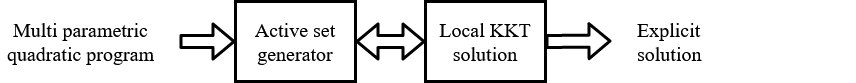
\includegraphics[width=.95\textwidth]{EMPC_PNG_Pics/MPQPAlgo.png}
%        \caption{Generic multi parametric quadratic program with explicit solver.}
%        \label{EMPC:fig:ControlStruct}
%    \end{figure}

\subsection{Storage of critical regions}\label{BASICCSR:sec:EMPCStorage}

The issue of iterative model based controllers is that they require a lot of computational resource. The CPU load and required ROM consumption could increase exponentially the longer the more steps the control horizon is calculated. For this reason explicit model bssed predictive controllers (EMPC) were developed, where only the storage the critical regions and the signal coefficients for each critical region, so the matrices $\textbf{H}$, $\mathcal{K}$, $\textbf{F}$, $\textbf{G}$ are required. The on-line part of control consists of searching the critical region for the current states and calculating the necessary inputs for them.
One method of storing entire critical regions in order to calculate them, and that is in the order in which the MP-LP or MP-QP problem is resolved. It has the disadvantage, that the search time can be high, as such starting from the top of the list, a linear search is not effective. The efficient method is to store critical regions already in a binary tree \cite{jones2006logarithmic}, \cite{tondel2003evaluation}, \cite{tondel2003constrained}, \cite{kutasi2008vector}. The method of generating the binary tree is shown in (Fig.\ref{BASICMPC:fig:searchtree}.).\\
 The basic idea is to sort the critical regions depending on their adjacent sides. For example, in (Fig.\ref{BASICMPC:fig:searchtree}.a.) side $j_1$ divides the state space into two, at the right of it are the regions $X_{2,3,4,5}$ and to the left are the regions $X_{1,2,6}$. They make up the nodes adjacent to the base node $I_1$ of the binary tree. Next the another side from the space is chosen defined by each node $I_2$ respectively $I_3$, and the algorithm is continued until all the regions in the current node correspond to the same control signal, denoted by $F$ on the shaft in fig. (Fig.\ref{BASICMPC:fig:searchtree}.b.) Thus with this search pattern logarithmic search time can be achieved.

 \begin{figure}[!ht]
        \centering
        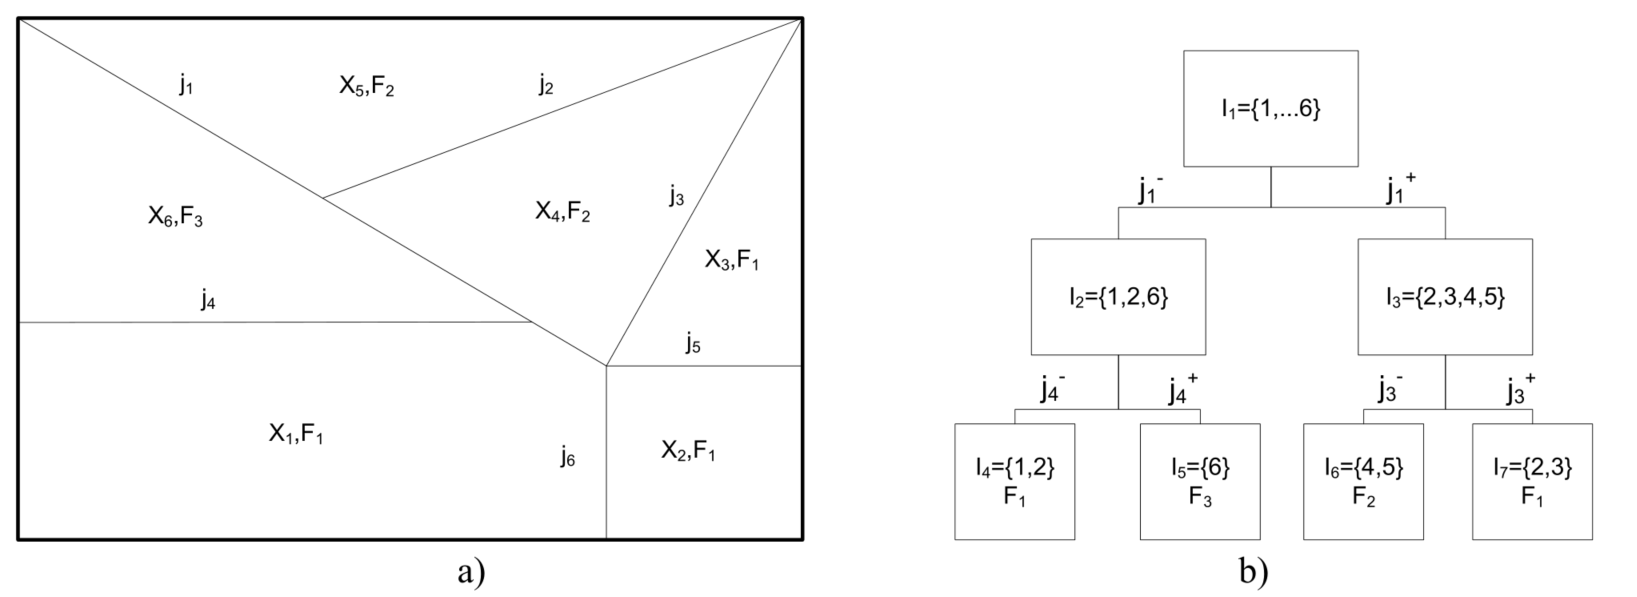
\includegraphics[width=\textwidth]{EMPC_PNG_Pics/BasicSearchTree.png}
        \caption{Basic search three of an EMPC where, a) are the critical regions for a space of 2D parameters,
b) the related binary tree.}
        \label{BASICMPC:fig:searchtree}
    \end{figure}

The implementation of MPC in explicit form is very efficient up to a certain number of critical regions, because they do not require calculations but only search in a table. For more complex problems or fast systems the method requires longer search time.
